\newpage
\def\thoigian{90}%--Thời gian
\de{Đề số 2}{Chương III. Hàm số bậc hai và đồ thị}



\begin{center}
	\textbf{PHẦN 1 - CÂU TRẮC NGHIỆM BỐN PHƯƠNG ÁN}
\end{center}
\Opensolutionfile{ans}[ans/ans-TN-ONTAPCHUONG-DE1]
\setcounter{ex}{0}
%Câu 1
\begin{ex}%[0D3N1-1]%[Dự án D - đợt 2 NH24-25- Lê Minh Thiện Anh]
	Một thiết bị đã ghi lại vận tốc $v$ (mét/giây) ở thời điểm $t$ (giây) của một vật chuyển động như trong bảng sau:
	\begin{center}\textcolor{black}{
	\begin{tabular}{|c|c|c|c|c|c|}
	\hline
	$t$ (giây)&$0{,}5$ &$1$ & $1{,}2$ & $1{,}8$  & $2{,}5$ \\
	\hline
	$v$ (mét/giây)&$1{,}5$ &$3$ & $0$ & $5{,}4$  & $7{,}5$ \\
	\hline
	\end{tabular}
	}\end{center}
	Khẳng định nào sau đây đúng?
	\choice
	{\True $v\left(0{,}5\right)=1{,}5$}
	{$v\left(0{,}5\right)=0{,}5$}
	{$v\left(0{,}5\right)=7{,}5$}
	{$v\left(0{,}5\right)=0$}
	\loigiai{
		Ta có $v\left(0{,}5\right)=1{,}5$.
}
\end{ex}

%Câu 2
\begin{ex}%[0D3N1-3]%[Dự án D - đợt 2 NH24-25- Lê Minh Thiện Anh]
	Cho hàm số $f(x)=\heva{&2 x-\sqrt{x+1}& &\text { khi }&& x \geq 1 \\& 5-x^2  &&\text { khi }&&  x<1}$. Giá trị $f(3)$ bằng
	\choice
	{ $8$}
	{$-4$}
	{$14$}
	{\True $4$}
	\loigiai{
		Ta có $f(3)=2\cdot 3-\sqrt{3+1}=4$.
}
\end{ex}

%Câu 3
\begin{ex}%[0D3H1-2]%[Dự án D - đợt 2 NH24-25- Lê Minh Thiện Anh]
	Tìm tập xác định $\mathscr{D}$ của hàm số $y=\sqrt{6-3 x}+\dfrac{x+3}{2 x^2-9 x+10}$.
	\choice
	{\True  $\mathscr{D}=(-\infty ; 2)$}
	{$\mathscr{D}=\mathbb{R} \setminus\left\{2 ; \dfrac{5}{2}\right\}$}
	{$\mathscr{D}=(2 ;+\infty) \setminus\left\{\dfrac{5}{2}\right\}$}
	{$\mathscr{D}=[2 ;+\infty) \setminus\left\{\dfrac{5}{2}\right\}$}
	\loigiai{
		Điều kiện xác định $\heva{&6-3x\geq 0\\&2x^2-9x+10\neq 0}\Leftrightarrow \heva{&x\leq 2\\&x\neq \dfrac{5}{2}\\&x\neq 2.}$\\
		Do đó tập xác định $\mathscr{D}$ của hàm số $y=\sqrt{6-3 x}+\dfrac{x+3}{2 x^2-9 x+10}$ là $\mathscr{D}=(-\infty ; 2)$.
}
\end{ex}

%Câu 4
\begin{ex}%ID%[Dự án D - đợt 2 NH24-25- Lê Minh Thiện Anh]
	\immini{Đồ thị hàm số $y=f(x)$ được cho như hình vẽ bên. Hàm số $y= f(x)$ đồng biến trên khoảng nào sau đây?
		\choice
		{\True $(1; +\infty) $}
		{$(0; +\infty) $}
		{$\mathbb{R} $}
		{$ (-1; +\infty)$}
		}
		{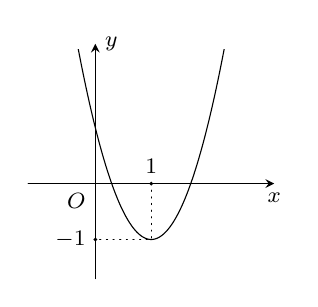
\begin{tikzpicture}[scale=0.71,>=stealth, font=\footnotesize, line join=round, line cap=round]
				\def\a{2} \def\b{-4} \def\c{1} % Hệ số
				\def\xmin{-1.2} \def\xmax{3.2}
				\def\ymin{-1.7} \def\ymax{2.5}
				\draw[->] (\xmin,0)--(\xmax,0) node [below]{$x$};
				\draw[->] (0,\ymin)--(0,\ymax) node [right]{$y$};
				\node at (0,0) [below left]{$O$};
				\clip (\xmin+0.1,\ymin+0.1) rectangle (\xmax-0.1,\ymax-0.1);
				\draw[smooth,samples=300] plot(\x,{\a*(\x)^2+\b*(\x)+\c});
				\draw[dotted] (1,0)|-(0,-1);
				\fill (1,0) circle (1pt) node [above] {$1$}
				(0,-1) circle (1pt) node [left] {$-1$};
				\end{tikzpicture}
		}
	\loigiai{
		Dựa vào đồ thị hàm số, ta thấy hàm số đồng biến trên khoảng $(1; +\infty)$.}
\end{ex}

%Câu 5
\begin{ex}%[0D3H1-3]%[Dự án D - đợt 2 NH24-25- Lê Minh Thiện Anh]
	Cho hàm số $f(x) =\heva{& \sqrt{x+1} &\text{nếu } x \ge 2\\ & x-2 & \text{nếu } x<2}$ có đồ thị $(C)$. Đồ thị $(C)$ đi qua điểm nào sau đây? 
	\choice
	{$M(-1;0) $}
	{\True $P(3;2) $}
	{$Q(4;2) $}
	{$N(2;0) $}
	\loigiai{
		Với $x=3$ thì $f(3)= \sqrt{3+1}=2 $ nên $P(3;2) \in (C).$}
\end{ex}

%Câu 6
\begin{ex}%[0D3N1-2]%[Dự án D - đợt 2 NH24-25- Lê Minh Thiện Anh]
	Tập xác định của hàm số $y=\sqrt{x-1}+\sqrt{2-x}$ là
	\choice
	{\True $\mathscr{D}=[1;2]$}
	{$\mathscr{D}=(-\infty;1]\cup[2;+\infty)$}
	{$\mathscr{D}=(-\infty;1)\cup (2;+\infty)$}
	{$\mathscr{D}=(1;2)$}
	\loigiai{
		Điều kiện xác định của hàm số $y=\sqrt{x-1}+\sqrt{2-x}$ là $\heva{&x-1\geqslant 0\\&2-x\geqslant 0} \Leftrightarrow 1\leqslant x\leqslant 2$.\\
		Vậy tập xác định của hàm số $y=\sqrt{x-1}+\sqrt{2-x}$ là $\mathscr{D}=[1;2]$.
}
\end{ex}

%Câu 7
\begin{ex}%[0D3N2-3]%[Dự án D - đợt 2 NH24-25- Lê Minh Thiện Anh]
	Trục đối xứng của parabol $y=x^2-4x-5$ là
	\choice
	{$x=-2$}
	{$x=-4$}
	{$x=4$}
	{\True $x=2$}
	\loigiai{
		Trục đối xứng của parabol là $x=\dfrac{-(-4)}{2\cdot1}=2$.
}
\end{ex}

%Câu 8
\begin{ex}%[0D3H2-2]%[Dự án D - đợt 2 NH24-25- Lê Minh Thiện Anh]
	Giá trị nhỏ nhất của hàm số $y=x^2-4x+1$ là
	\choice
	{\True $-3$}
	{$1$}
	{$3$}
	{$13$}
	\loigiai{
		Ta có $x^2-4x+1=x^2-4x+4-3=\left(x-2\right)^2-3\geqslant-3$. \\
		Dấu \lq\lq$=$\rq\rq\ xảy ra khi $x=2$. \\
		Vậy giá trị nhỏ nhất của hàm số $y=x^2-4x+1$ bằng $-3$ khi $x=2$.
}
\end{ex}

%Câu 9
\begin{ex}%[0D3N2-1]%[Dự án D - đợt 2 NH24-25- Lê Minh Thiện Anh]
	Hàm số nào dưới đây là hàm số bậc hai?
	\choice
	{$y=-2x+3$}
	{\True $y=2x^2-4x$}
	{$y=\dfrac{1}{x^2}+2x-3$}
	{$y=-x^2+\dfrac{2}{x}+2$}
	\loigiai{
		Hàm số bậc hai là $y=2x^2-4x$.
}
\end{ex}

%Câu 10
\begin{ex}%[0D3N2-2]%[Dự án D - đợt 2 NH24-25- Lê Minh Thiện Anh]
	Tọa độ đỉnh của parabol $y=-2x^2-4x+6$ là
	\choice
	{\True $I\left(-1;8\right)$}
	{$I\left(1;0\right)$}
	{$I\left(2;-10\right)$}
	{$I\left(-1;6\right)$}
	\loigiai{
		Hoành độ đỉnh $I$ là $x=-\dfrac{b}{2a}=-1$ nên tọa độ đỉnh $I\left(-1;8\right)$.
}
\end{ex}

%Câu 11
\begin{ex}%[0D3H2-2]%[Dự án D - đợt 2 NH24-25- Lê Minh Thiện Anh]
	Bảng biến thiên sau đây là bảng biến thiên của hàm số nào?
	\begin{center}
	\begin{tikzpicture}
	\tkzTabInit[nocadre=false,lgt=1.2,espcl=2.5,deltacl=0.6]
	{$x$ /0.6, $y$ /2.5}
	{$-\infty$,$2$,$+\infty$}
	%\tkzTabLine{,-,d,-,}
	\tkzTabVar{-/$-\infty$,+/$-4$,-/$-\infty$}
	\begin{scope}[on background layer]\path[white]node{MDD-904};\end{scope}
	\end{tikzpicture}
	\end{center}
	\choice
	{ $ y=x^2+4 x$}
	{$y=-x^2-4 x$}
	{$y=-x^2-4 x+8$}
	{\True $y=-x^2-4 x-8$}
	\loigiai{
	Nhánh bên phải của đồ thị hàm số đi xuống nên $a<0$. Loại $ y=x^2+4 x$.\\
	Toạ độ đỉnh $(-2;-4)$ nên loại $y=-x^2-4 x$ và $y=-x^2-4 x+8$.
}
\end{ex}

%Câu 12
\begin{ex}%[0D3H2-2]%[Dự án D - đợt 2 NH24-25- Lê Minh Thiện Anh]
	\immini{Cho hàm số $y=ax^2+bx+c$ có đồ thị như hình dưới đây. Khẳng định nào sau đây \textbf{đúng}?}{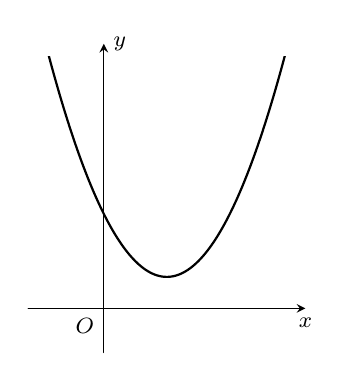
\begin{tikzpicture}[scale=0.8, font=\footnotesize, line join=round, line cap=round, >=stealth]
			\def\xmin{-1}\def\xmax{3}\def\ymin{-0.5}\def\ymax{4}
			\draw[->] (\xmin-0.2,0)--(\xmax+0.2,0) node[below] {\footnotesize $x$};
			\draw[->] (0,\ymin-0.2)--(0,\ymax+0.2) node[right] {\footnotesize $y$};
			\draw (0,0) node [below left] {\footnotesize $O$};
			\foreach \x in {}\draw (\x,0.1)--(\x,-0.1) node [below] {\footnotesize $\x$};
			\foreach \y in {}\draw (0.1,\y)--(-0.1,\y) node [left] {\footnotesize $\y$};
			\clip (\xmin,\ymin) rectangle (\xmax,\ymax);
			\draw[thick,smooth,samples=200,domain=\xmin:\xmax] plot (\x,{1*((\x)^2)+-2*\x+3/2});
	\end{tikzpicture}}
	\choice
	{\True $a>0$, $b<0$, $c>0$}
	{$a>0$, $b>0$, $c<0$}
	{$a>0$, $b<0$, $c<0$}
	{$a<0$, $b<0$, $c>0$}
	\loigiai{
		Nhận xét
		\begin{itemize}
			\item Đồ thị hàm số có bề lõm quay lên trên nên $a>0$.
			\item Đồ thị hàm số cắt trục tung tại điểm nằm phía trên trục $Ox$ nên $c>0$.
		\end{itemize}
	}
\end{ex}
\Closesolutionfile{ans}
%\begin{center}
%	\textbf{ĐÁP ÁN}
%	\inputansbox{10}{ans/ans}	
%\end{center}



\begin{center}
	\textbf{PHẦN 2 - CÂU TRẮC NGHIỆM ĐÚNG SAI}
\end{center}
\setcounter{ex}{0}
\Opensolutionfile{ans}[ans/answer-DS-ONTAPCHUONG-DE2]
\begin{ex}%[0D3H1-3]%[Dự án D - đợt 2 NH24-25- Lê Minh Thiện Anh]
	Cho hàm số $y=x^2-2x$ có đồ thị $(P)$.
	\choiceTF
	{\True Hàm số có tập xác định $\mathscr{D}=\mathbb{R}$}
	{Điểm $(0;0)$ và $(2;2)$ thuộc đồ thị hàm số đã cho}
	{\True Điểm $M(x;y)\in(P)$ sao cho biểu thức $T = 2x - y + 5$ đạt giá trị lớn nhất thì giá trị lớn nhất đó bằng $9$}
	{Đường thẳng $y=-x+2$ cắt $(P)$ tại hai điểm $A$, $B$ thì diện tích tam giác $OAB$ bằng $4$}
	\loigiai{
		\begin{itemchoice}
			\itemch Hàm số có tập xác định $\mathscr{D}=\mathbb{R}$
			\itemch 
			Điểm $(2;2)$ không thuộc đồ thị hàm số vì $2=2^2-2\cdot2$ (sai).
			\itemch 
			Điểm $M(x; y)$ thuộc $(P): y = x^2 – 2x$.
			Ta thay $y = x^2 – 2x$ vào biểu thức $T$ ta được $$T = –x^2 + 4x + 5=-x^2+4x-4+9=-(x-2)^2+9.$$
			Giá trị lớn nhất của $T$ đạt được khi $x = 2\Rightarrow y=0$.\\
			Vậy biểu thức $T = 2x - y + 5$ đạt giá trị lớn nhất bằng $9$ tại điểm $M(2; 0)$ trên parabol $(P)$.
			\itemch 
			Phương trình hoành độ giao điểm của $(d): y = -x + 2$ và $(P): y = x^2 – 2x$ là
			$$x^2 – 2x = -x + 2\Leftrightarrow x^2 – x – 2 = 0\Leftrightarrow \hoac{&x=2\\&x=-1.}$$
			Ta tìm được hai điểm $A(2;0)$ và $B(-1;3)$.\\
			Ta thấy điểm $A(2; 0)$ nằm trên trục hoành $Ox$. Vậy ta có thể chọn cạnh $OA$ làm đáy của tam giác.\\
			Độ dài đoạn $OA$ là $OA=\left|x_A - x_O\right| = \left|2 - 0\right| = 2$.\\
			Chiều cao của tam giác ứng với đáy $OA$ là khoảng cách từ điểm $B$ đến trục hoành $Ox$. Khoảng cách này chính là giá trị tuyệt đối của tung độ điểm $B$ và ta có $h=3$.\\
			Vậy
			$S_{\triangle OAB} = \dfrac{1}{2}OA\cdot h = \dfrac{1}{2}\cdot 2 \cdot 3 = 3$.
	\end{itemchoice}}
\end{ex}

\begin{ex}%[0D3H2-2]%[Dự án D - đợt 2 NH24-25- Lê Minh Thiện Anh]
	Cho hàm số $y=f(x)=2x^2+4x-6$ có đồ thị là parabol $(P)$.
	\choiceTF
	{\True Trục đối xứng của $(P)$ là $x=-1$ }
	{\True Giá trị nhỏ nhất của hàm số là $-8$}
	{\True Đồ thị cắt $Ox$ tại hai điểm $A$, $B$ cắt $Oy$ tại $C$, đường tròn $(C)$ qua $A$, $B$, $C$ cắt $(P)$ tại $D$ có tọa độ $(-2;-6)$}
	{Có đúng $8$ giá trị nguyên âm của tham số $m$ để phương trình $2x^2 + 4x – 6 = m$ có đúng $2$ nghiệm thực phân biệt}
	\loigiai{
		\begin{itemchoice}
			\itemch 
			Trục đối xứng của $(P)$ là $x=-\dfrac{4}{2\cdot 2}$ hay $x=-1$.
			\itemch 
			Đồ thị hàm số $y=f(x)=2x^2+4x-6$ có tọa độ đỉnh là $S(-1;-8)$ nên giá trị nhỏ nhất của hàm số bằng $-8$ tại $x=-1$.
			\itemch 
			Đồ thị cắt $Ox$ tại hai điểm $A(-3;0)$, $B(1;0)$ cắt $Oy$ tại $C(0;-6)$.\\
			Vì $A(-3;0)$, $B(1;0)$ nằm trên $Ox$ vừa thuộc $(P)$ vừa thuộc $(C)$ đối xứng nhau qua trục đối xứng nên $D$ cũng đối xứng với $C(0;-6)$ qua trục đối xứng.\\
			Ta có trục đối xứng $x=-1$ nên $D(-2;-6)$.
			\itemch 
			Ta có bảng biến thiên
			\begin{center}
				
\begin{tikzpicture}
					\tkzTabInit[nocadre=true, lgt=1, espcl=4, deltacl=0.5] 
					{$x$/0.7,$y$/2}
					{$-\infty$,$-1$,$+\infty$}
					\tkzTabVar{+/$+\infty$,-/$-8$,+/$+\infty$}
				\end{tikzpicture}
			\end{center}
			Đồ thị hàm số $y=f(x)$ là 
			\begin{center}
			\begin{tikzpicture}[>=stealth,scale=0.5, line join=round, line cap=round]
					\draw[->] (-5,0)--(3,0) node [below]{$x$};
					\draw[->] (0,-9)--(0,3) node [left]{$y$};
					\node at (0,0) [below left]{$O$};
					\draw[dashed] (-1,0) node[above] {$-1$} -- (-1,-8)--(0,-8)node[right] {$-8$};
					\path (-3.2,2) node[left] {$y=f(x)$};
					\path (2.5,-3.5) node[right] {$y=m$};
					\draw (-5,-4)--(3,-4);
					\clip (-5,-9) rectangle (3,3);
					\draw[smooth,samples=300] plot (\x,{2*(\x)^2+4*(\x)-6});
			\end{tikzpicture}
			\end{center}			
			Dựa vào đồ thị để phương trình có đúng $2$ nghiệm thực phân biệt, điều kiện của $m$ là $m>-8$.\\
			Vì đề bài yêu cầu tìm các giá trị nguyên âm của $m$, nên các giá trị thỏa mãn là $m \in \{-7; -6; -5; -4; -3; -2; -1\}$.\\
			Có tổng cộng $7$ giá trị nguyên của $m$.
		\end{itemchoice}
	} 
\end{ex}

\Closesolutionfile{ans}
%\inputansbox[2]{2}{ans/answer.tex}
\begin{center}
\textbf{PHẦN 3 - CÂU TRẮC NGHIỆM TRẢ LỜI NGẮN}
\end{center}
\setcounter{ex}{0}
\Opensolutionfile{ans}[ans-KQ-ONTAPCHUONG-DE2]
\setcounter{ex}{0}
\begin{ex}%[0D3N1-3]%[Dự án D - đợt 2 NH24-25- Lê Minh Thiện Anh]
	Cho hàm số $y=\heva{&\dfrac{2}{x-1}, &x \in(-\infty; 0) \\
		&\sqrt{x+1}, &x \in[0;+\infty)}$. Giá trị $f(0)+f(-1)$ bằng bao nhiêu?
		
	\shortans[oly]{$0$}
	\loigiai{
		Với $x=0$ ta có $f(0)=\sqrt{0+1}=1$.\\
		Với $x=-1$ ta có $f(-1)=-1$.\\
		Vậy $f(0)+f(-1)=0$.}
\end{ex}

\begin{ex}%[0D3V1-3]%[Dự án D - đợt 2 NH24-25- Lê Minh Thiện Anh]
	Bảng niêm yết giá cước của một hãng taxi như sau:
	\begin{center}
	\begin{tabular}{|c|c|c|}
	\hline
	Giá mở cửa	&Giá km tiếp theo &Từ km thứ $26$\\
	\hline
	$14\,000$ đ/$0{,}8$km	&$16\,300$ đ/km &$13\,300$ đ/km \\
	\hline
	\end{tabular}
	\end{center}
	Bác An đi taxi và cần di chuyển quãng đường $20$ km. Hỏi bác An phải trả bao nhiêu tiền?
	(kết quả làm tròn tới hàng nghìn, đơn vị: nghìn đồng).
	
	\shortans[oly]{$327$}
	\loigiai{
		Cần chi $14\,000$ đồng cho $0{,}8$ km đầu tiên;\\
		$16\,300\cdot (20-0,8)=312\,960$ đồng cho những km tiếp theo của quãng đường $20$ km.\\
		Tổng số tiền bác An phải trả là $14\,000 + 312\,960 = 326\,960$ đồng.}
\end{ex}

\begin{ex}%ID%[Dự án D - đợt 2 NH24-25- Lê Minh Thiện Anh]
	Cho parabol $(P)\colon y=ax^2+b x-4$ và trục đối xứng $x=-2$ và đi qua điểm $A\left(1;6\right)$. Tính $b-a$.

	\shortans[oly]{6}
	\loigiai{
		Trục đối xứng $x=-2\Rightarrow-\dfrac{b}{2a}=-2\Leftrightarrow 4a-b=0$.\\
		$(P)$ đi qua điểm $A(1;6)$ nên thay $x=1$, $y=6$ vào phương trình $(P)$ suy ra \[a+b-4=6\Leftrightarrow a+b=10.\]
		Vậy ta có hệ phương trình $\heva{& 4a-b=0 \\ & a+b=10}\Leftrightarrow\heva{& a=2 \\ & b=8.}$\\
		Vậy $b-a=8-2=6$.
	}
\end{ex}

\begin{ex}%ID%[Dự án D - đợt 2 NH24-25- Lê Minh Thiện Anh]
	Có bao nhiêu giá trị nguyên dương của tham số $m$ để hàm số $y=-x^2+2(3m-6)x+3-5m$ nghịch biến trên khoảng $(6;2\,023)$?
	
	\shortans[oly]{$4$}
	\loigiai{
		Hàm số đã cho là hàm số bậc hai có hệ số $a<0$ nên nó nghịch biến trên khoảng $(3m-6;+\infty)$.\\
		Để thỏa mãn yêu cầu bài toán thì phải có $3m-6\le 6$ hay $m\le 4$.\\
		Vậy có bốn giá trị nguyên dương của $m$ thỏa mãn, đó là $1$, $2$, $3$, $4$.}
\end{ex}

\Closesolutionfile{ans}
\begin{center}
	\textbf{PHẦN 4 - TỰ LUẬN}
\end{center}
\setcounter{ex}{0}
%Câu 1...........................
\begin{ex}%[0D3V1-7]%[Dự án D - đợt 2 NH24-25- Lê Minh Thiện Anh]
	Hiện nay, giá tiền điện sinh hoạt của 1 kWh điện sẽ được tính theo bậc lũy tiến. Có tổng cộng 6 bậc, mức sử dụng càng nhiều thì giá tiền 1 kWh sẽ càng cao. Cụ thể
	\begin{center}
	\begin{tabular}{|l|c|}
	\hline
	\multicolumn{1}{|c|}{Giá bán lẻ điện sinh hoạt} & Giá bán điện (đồng/kWh) \\ \hline
	Bậc 1: Cho kWh từ 0-50                          & 1806                    \\ \hline
	Bậc 2: Cho kWh từ 51-100                        & 1866                    \\ \hline
	Bậc 3: Cho kWh từ 101-200                       & 2167                    \\ \hline
	Bậc 4: Cho kWh từ 201-300                       & 2729                    \\ \hline
	Bậc 5: Cho kWh từ 301-400                       & 3050                    \\ \hline
	Bậc 6: Cho kWh từ 401 trở lên                   & 3151                    \\ \hline
	\end{tabular}
	\end{center}
	Gọi $x$ là lượng điện tiêu thụ (đơn vị kWh) và $y$ là số tiền phải trả tương ứng (đơn vị nghìn đồng). Tìm công thức mô tả sự phụ thuộc của $y$ vào $x$ khi $200<x\le 300$.
	\loigiai{
		Số tiền phải trả cho $50$ kWh đầu tiên là $50\cdot1{,}806=90{,}3$ nghìn đồng.\\
		Số tiền phải trả cho $5$ kWh tiếp theo là $50\cdot1{,}866=93{,}3$ nghìn đồng.\\
		Số tiền phải trả cho $100$ kWh tiếp theo là $100\cdot2{,}167=216{,}7$ nghìn đồng.\\
		Số tiền phải trả cho $x$ kWh tiếp theo là $x\cdot2{,}729=2{,}729x$ nghìn đồng.\\
		Tổng số tiền phải trả là $y=2{,}729x+216{,}7+93{,}3+90{,}3=2{,}729x+400{,}3$ nghìn đồng.
}
\end{ex}

%Câu 2...........................
\begin{ex}%[0D3H2-1]%[Dự án D - đợt 2 NH24-25- Lê Minh Thiện Anh]
	Cho parabol $(P)\colon y=ax^2+bx+2$. Tìm $a$, $b$ biết $(P)$ có đỉnh là $S(-2;-2)$.
	\loigiai{
		Điều kiện: $a \neq 0$.\\
		$(P)$ có đỉnh $S(-2;-2)$ nên ta có hệ $\left\{\begin{aligned} &-\dfrac{b}{2a}=-2 \\ &-2=a \cdot (-2)^2+b \cdot (-2)+2 \end{aligned}\right.
		\Leftrightarrow \left\{\begin{aligned} &a=1\\&b=4. \end{aligned}\right.$\\
		Vậy $a=1$; $b=4$.
}
\end{ex}

%Câu 3...........................
\begin{ex}%[0D3C2-6]%[Dự án D - đợt 2 NH24-25- Lê Minh Thiện Anh]
	Cầu Đông Trù là một cây cầu bắc qua sông Đuống, được xây dựng theo kiểu vòm ống thép, cầu gồm $3$ nhịp chính trong đó $2$ nhịp biên dài $80$ m và nhịp giữa sông dài $120$ m. Mỗi nhịp được kiến trúc bằng đường cong tựa như một parabol. Giả sử rằng mỗi nhịp của cầu là một parabol (tham khảo hình vẽ). Một người đã dùng dây dọi (không giãn) gắn lên thành cầu ở vị trí $B$ và điều chỉnh độ dài dây dọi đề quả nặng vừa chạm đất ở vị trí $H$ (khi lặng gió), sau đó đo được chiều dài đoạn dây dọi $BH$ sử dụng là $2{,}9$ m và khoảng cách từ chân trụ cầu đến quả nặng (đoạn $OH$) là $3$ m. Gọi khoảng cách từ đỉnh $S$ vòm đến mặt đường là $h$. Nếu dùng dữ liệu thu thập được và tính toán thì người này sẽ ước tính được độ cao $h$ là bao nhiêu? (kết quả làm tròn đến hàng đơn vị).
\begin{minipage}{.5\textwidth}
\centering
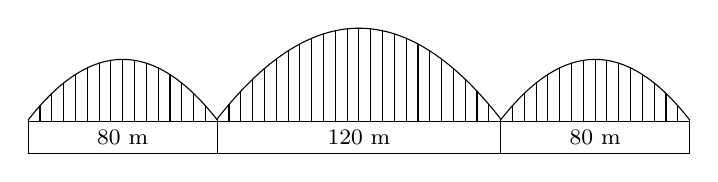
\begin{tikzpicture}[scale=.4, xscale=.75, font=\footnotesize, line join=round, line cap=round, >=stealth]
	\def\a{14}
	\pgfmathsetmacro\b{3*\a/7}
	\def\f(#1){-0.08*(#1)^2+2.97}
	\draw (-\a,0)--(\a,0) (-\a,-1)--(\a,-1);
	\foreach \i in {-\a,-\b,\b,\a}  \draw (\i,0)--(\i,-1);
	\tikzset{cau/.pic={
		\draw[domain=-\b:\b, samples=100, scale=.4, xscale=.75]plot (\x, {\f(\x)});
	}}
	\tikzset{day1/.pic={
		\foreach \m in {-6,-5.5,...,6} \draw[scale=.4, xscale=.75] (\m,{\f(\m)})--(\m,0);
	}}
	\tikzset{day2/.pic={
		\foreach \m in {-6,-5.25,...,6} \draw[scale=.4, xscale=.75] (\m,{\f(\m)})--(\m,0);
	}}
	\draw (0,0) pic{cau} pic{day1};
	\draw (-10,0) pic[scale=2/3]{cau} pic[scale=2/3]{day2};
	\draw (10,0) pic[scale=2/3]{cau} pic[scale=2/3]{day2};
	\draw (0,-0.5) node{$120$ m} (-10,-0.5) node{$80$ m} (10,-0.5) node{$80$ m};
\end{tikzpicture}
\centering{\it Hình minh họa cầu Đông Trù}
\end{minipage}%
\begin{minipage}{.5\textwidth}
\centering
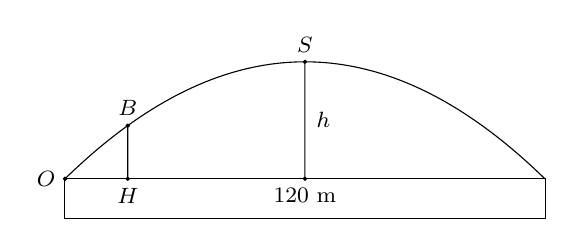
\begin{tikzpicture}[scale=.5, font=\footnotesize, line join=round, line cap=round, >=stealth]
	\def\a{14}
	\pgfmathsetmacro\b{3*\a/7}
	\def\f(#1){-0.08*(#1)^2+2.97}
	\tikzset{cau/.pic={
		\draw[domain=-\b-0.1:\b+0.1, samples=100, scale=.5]plot (\x, {\f(\x)});
	}}
	\draw (0,0) pic{cau};
	\draw (-\b-0.1,0)--(-\b-0.1,-1)--(\b+0.1,-1)--(\b+0.1,0)--cycle;
	\draw 	(-4.5,{\f(-4.5)}) node[above]{$B$}circle (1.2pt) -- (-4.5,0) node[below]{$H$} circle (1.2pt)
			(0,2.97) node[above]{$S$}circle (1.2pt)-- (0,0)circle (1.2pt);
	\draw[fill=black] (-6.09,0) node[left]{$O$}circle (1.2pt) (0.05, 1.5) node[right]{$h$} (0,0)node[below]{$120$ m};
\end{tikzpicture}\\
\centering{\it Hình minh họa nhịp giữa cầu Đông Trù}
\end{minipage}
\loigiai{
	\immini{Chọn hệ trục tọa độ $Oxy$ như hình vẽ. Gọi parabol $(P)\colon y=ax^2+bx+c$ $(a<0)$.\\
		Vì $(P)$ đi qua gốc $O$ nên $c=0$.\\
		Trục của $(P)$ là đường thẳng $x=60$ nên $\dfrac{-b}{2a}=60 \Leftrightarrow b=-120a$.\\
		Vì $B(3;2{,}9) \in (P)$ nên $2{,}9=9a+3b$. Thay $b=-120a$, ta được
		$$2{,}9=9a+3\cdot (-120a) \Leftrightarrow a=-\dfrac{29}{3510}.$$
	}{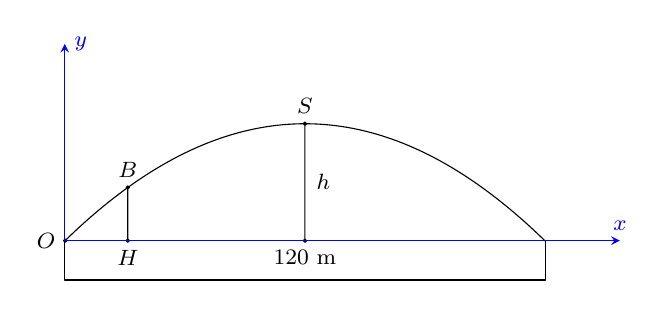
\begin{tikzpicture}[scale=.5, font=\footnotesize, line join=round, line cap=round, >=stealth]
		\def\a{14}
		\pgfmathsetmacro\b{3*\a/7}
		\def\f(#1){-0.08*(#1)^2+2.97}
		\tikzset{cau/.pic={
		\draw[domain=-\b-0.1:\b+0.1, samples=100, scale=.5]plot (\x, {\f(\x)});}}
		\draw (0,0) pic{cau};
		\draw (-\b-0.1,0)--(-\b-0.1,-1)--(\b+0.1,-1)--(\b+0.1,0)--cycle;
		\draw 	(-4.5,{\f(-4.5)}) node[above]{$B$}circle (1.2pt) -- (-4.5,0) node[below]{$H$} circle (1.2pt)
		(0,2.97) node[above]{$S$}circle (1.2pt)-- (0,0)circle (1.2pt);
		\draw[fill=black] (-6.09,0) node[left]{$O$}circle (1.2pt) (0.05, 1.5) node[right]{$h$} (0,0)node[below]{$120$ m};
		\draw[->,blue] (-6.1,0)--(8,0)node[above]{$x$};
		\draw[->,blue] (-6.1,0)--(-6.1,5)node[right]{$y$};
		%\draw[fill=black] (6.1,0)node[above]{$60$} circle (1.2pt);
	\end{tikzpicture}
	}
	Do đó $(P)\colon y=-\dfrac{29}{3510}x^2+\dfrac{116}{117}x$.\\ 
	Hoành độ điểm $S$ là $x=60$ và tung độ điểm $S$ là $y=-\dfrac{29}{3510}\cdot 60^2+\dfrac{116}{117}\cdot 60=\dfrac{1160}{39}$. Vậy $h \approx 30$ m.
}
\end{ex}

